\section{Arduinoen og programmering} \label{sec:arduino}
\subsection{Arduino som komponent}
%--------------- Indsæt en arduino ---------------%
\begin{figure}[H]
	\centering
    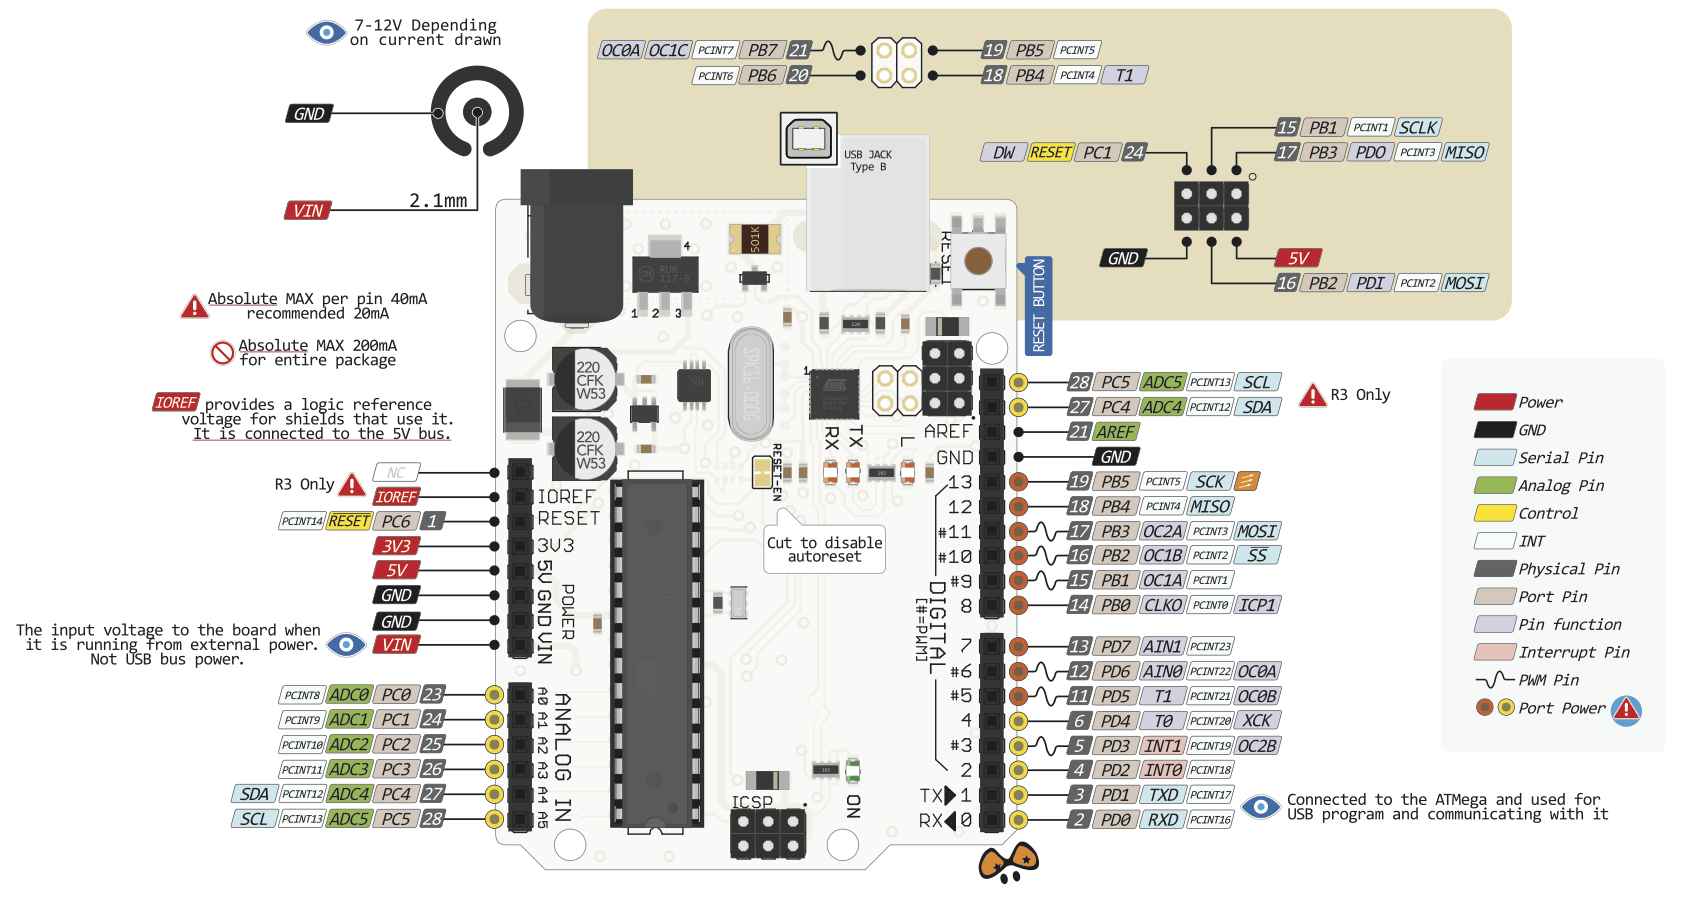
\includegraphics[width=\textwidth]{figures/arduino/portmani.PNG}
	\caption{Arduino uno med ATmega328}
	\label{fig:portmani}
	Her kan man se hvilke ben der er på Arduinoen, og hvilke porte de fordelt på ( PORTB, PORTC og PORTD). Hvis man ser på "Port pin", står der P for port, efterfulgt af bogstavet for hvilken port den er tildelt, efterfulgt af dens bit position i den port.\\
	Vi har også opgivet den påkrævede spænding for at køre Arduinoen. Vi kan også se Analog input ben (A0-A5) og de digital input og output ben (0-13). Vi kan se ud fra analog ben A4 og A5 at de er SDA og SCL, som er relevant når vi skal benytte I2C kredsen.
	\\Kilde: \url{http://pighixxx.com/unov3pdf.pdf}
\end{figure}
\subsubsection{Analog inputs og outputs (PWM)}\label{sec:ard:analog}
Analog input i Arduinoen er et input som beskriver spændingsfaldet over inputtet og jord med et 10 bit tal.\cite{arduinoAnalog} Dette betyder at den laveste værdi og højeste værdi af et analog input er
\begin{align}
\SI{}{U_{MIN}}&=b00\,0000\,0000\rightarrow 0\rightarrow \SI{0}{V}\\
\SI{}{U_{MAX}}&=b11\,1111\,1111\rightarrow 1023\rightarrow \SI{5}{V}\\
\end{align}
Med Arduinoen kan man få et analog input igennem en analog ben (se \ref{fig:portmani}), og kalde metoden \emph{analogRead()} til benets nummer, eksempelvis A0. Da vores precision er på 10 bit, til at beskrive et maks spændingsfald på $\SI{5}{V}$, må det gælde at den laveste ændring i spændingsfaldet vi kan måle er
\begin{align}
U_{prec}&=\frac{\SI{5}{V}}{1023}\approx \SI{5d-3}{V}
\end{align}
\subsubsection{Digital inputs og outputs}
Digital input på Arduinoen er en boolean værdi, som enden kan være sand eller falsk (også kendt som TRUE/FALSE eller HIGH/LOW). Disse værdier reflektere den digitale logik på det digitale ben, som fungere således: når spændingsfaldet mellem bennet og jord er $\SI{5}{V}$ er værdien sand og når spændingsfaldet er $\SI{0}{V}$ er den falsk. Mere præcist skifter værdien mellem at være sand og falsk ved omkring $\SI{3}{V}$, på $\SI{5}{V}$ logik Arduinoer. \cite{arduino:dig}\\
\\
Et digital output følger samme logik, her der sætter man dog udgangsspændingen på bennet. Det betyder altså at hvis man sætter et digital ben til sandt, vil udgangsspændingen på bennet være $\SI{5}{V}$ og hvis man sætter det til falsk vil det være $\SI{0}{V}$. \cite{arduino:dig}\\
\\


\subsubsection{I2C - Synkroniseret kommunikation}


%-------------------------------------------------------------------------------------------------------------------------------------------
%--------------------------------------- PROGRAMMING PART ----------------------------------------------------------------------------------
%-------------------------------------------------------------------------------------------------------------------------------------------
\subsection{Kort beskrivelse af programmets formål}
\subsubsection{Master Arduino}
Vores Master Arduino står for styring af motorerne, ladningssensor og hastighedssensor. Programmet til Master Arduinoen skal kunne kommunikere med Controlleren, så den kan se om der skal rygges op eller ned på kanonen eller om der skal affyres. Den skal også kunne bestemme farven af bolden i røret og om der faktisk er en bold i røret. Når bolden bliver affyret skal hastigheden af bolden også kunne bestemmes. Til sidst skal den kunne sende information som farven af bolden, hældningen af kanonen og hastigheden af bolden til Controlleren, så det kan skrives på displayet.
\subsubsection{Controller Arduino}
Controller Arduinoen skal kunne sende data om knappernes tilstand og kunne modtage data om hvad der skal stå på displayet. Da vores bruger benytter Controlleren til at styre kanonen, skal forsinkelsen imellem at man trykker på en knap, til at kanonen ryger sig være relativ lille.\\
\\
\\
\\
Programmet til master Arduinoen kan fines i bilag \ref{bilag:programMaster} og Controller Arduinoen i bilag \ref{bilag:programController}, som er kommenteret. De mest komplekse og primære funktioner vi har programmeret, er beskrevet i sektion \ref{sec:primaerefunc}.
\subsection{Oversigt over inputs og outputs og lokation}
\begin{table}[H]
	\caption{Inputs og outputs for Master Arduinoen} % title
	\label{tab:IOMaster}
	\centering
		\begin{tabular}{c|c c} 
		Ben & I/O & Forbundet komponent\\ [0.5ex] 
		\hline 
			2 & Output & Stepper motor\\
			3 & Output & Stepper motor\\
			4 & Output & Stepper motor\\
			5 & Output & Stepper motor\\
			6 & Output & Trækmotor\\
			9 & Output & Gearmotor (fri)\\
			10 & Output & Gearmotor (lås)\\
			11 & Output & Ladningssensor LED (grøn)\\
			12 & Output & Ladningssensor LED (rød)\\
			13 & Output & Ladningssensor LED (blå)\\
			A0 & Input & Ladningssensor Fotodiode\\
			A1 & Input & Hastighedssensor 1\\			
			A2 & Input & Hastighedssensor 2\\
			A4 (SDA) & I/O & I2C kommunikation (data)\\
			A5 (SCL) & I/O & I2C kommunikation (clock)\\[1ex]
		\hline %inserts single line
	\end{tabular}
\end{table}

\begin{table}[H]
	\caption{Inputs og outputs for Controller Arduinoen} % title
	\label{tab:IOController}
	\centering
		\begin{tabular}{c|c c} 
		Ben & I/O & Forbundet komponent\\ [0.5ex] 
		\hline 
			2 & I/O & LCD (DB7)\\
			3 & I/O & LCD (DB6)\\
			4 &I/O & LCD (DB5)\\
			5 &I/O & LCD (DB4)\\
			11 & Output & LCD (E)\\
			12 &Output & LCD (RS)\\
			A0 & Input & Knap (ryg kanon op)\\
			A1 & Input & Knap (ryg kanon ned)\\			
			A2 & Input & Knap (affyre bold)\\
			A4 (SDA) & I/O & I2C kommunikation (data)\\
			A5 (SCL) & I/O & I2C kommunikation (clock)\\[1ex]
		\hline %inserts single line
	\end{tabular}
\end{table}
\todo{ret det med I2C ben}
\subsection{Primære funktioner}\label{sec:primaerefunc}
\subsubsection{1}
\subsubsection{2}
\subsubsection{3}